
%%%%%%%%%%%%%%%%%%%%%%%%%%%%%%%%%%%%%%%%%%%%%%%%%%%%%%%%%%%%%%%%%%%%%
%% This is a (brief) model paper using the achemso class
%% The document class accepts keyval options, which should include
%% the target journal and optionally the manuscript type.
%%%%%%%%%%%%%%%%%%%%%%%%%%%%%%%%%%%%%%%%%%%%%%%%%%%%%%%%%%%%%%%%%%%%%
\documentclass[journal=jacsat,manuscript=article]{achemso}

%%%%%%%%%%%%%%%%%%%%%%%%%%%%%%%%%%%%%%%%%%%%%%%%%%%%%%%%%%%%%%%%%%%%%
%% Place any additional packages needed here.  Only include packages
%% which are essential, to avoid problems later. Do NOT use any
%% packages which require e-TeX (for example etoolbox): the e-TeX
%% extensions are not currently available on the ACS conversion
%% servers.
%%%%%%%%%%%%%%%%%%%%%%%%%%%%%%%%%%%%%%%%%%%%%%%%%%%%%%%%%%%%%%%%%%%%%
\usepackage[version=3]{mhchem} % Formula subscripts using \ce{}
\usepackage[T1]{fontenc}       % Use modern font encodings

%%%%%%%%%%%%%%%%%%%%%%%%%%%%%%%%%%%%%%%%%%%%%%%%%%%%%%%%%%%%%%%%%%%%%
%% If issues arise when submitting your manuscript, you may want to
%% un-comment the next line.  This provides information on the
%% version of every file you have used.
%%%%%%%%%%%%%%%%%%%%%%%%%%%%%%%%%%%%%%%%%%%%%%%%%%%%%%%%%%%%%%%%%%%%%
%%\listfiles

%%%%%%%%%%%%%%%%%%%%%%%%%%%%%%%%%%%%%%%%%%%%%%%%%%%%%%%%%%%%%%%%%%%%%
%% Place any additional macros here.  Please use \newcommand* where
%% possible, and avoid layout-changing macros (which are not used
%% when typesetting).
%%%%%%%%%%%%%%%%%%%%%%%%%%%%%%%%%%%%%%%%%%%%%%%%%%%%%%%%%%%%%%%%%%%%%
\newcommand*\mycommand[1]{\texttt{\emph{#1}}}
\usepackage{color}
\def\todo#1{{\color{red}[TODO: #1]}}




%%%%%%%%%%%%%%%%%%%%%%%%%%%%%%%%%%%%%%%%%%%%%%%%%%%%%%%%%%%%%%%%%%%%%
%% Meta-data block
%% ---------------
%% Each author should be given as a separate \author command.
%%
%% Corresponding authors should have an e-mail given after the author
%% name as an \email command. Phone and fax numbers can be given
%% using \phone and \fax, respectively; this information is optional.
%%
%% The affiliation of authors is given after the authors; each
%% \affiliation command applies to all preceding authors not already
%% assigned an affiliation.
%%
%% The affiliation takes an option argument for the short name.  This
%% will typically be something like "University of Somewhere".
%%
%% The \altaffiliation macro should be used for new address, etc.
%% On the other hand, \alsoaffiliation is used on a per author basis
%% when authors are associated with multiple institutions.
%%%%%%%%%%%%%%%%%%%%%%%%%%%%%%%%%%%%%%%%%%%%%%%%%%%%%%%%%%%%%%%%%%%%%

\author{Robert O. Ness}
\email{nessr@purdue.edu}
\affiliation[Purdue University]{Purdue University Department of Statistics, West Lafayette}
\alsoaffiliation[Northeastern University]{College of Science, College of Computer and Information Science, Northeastern University, Boston}
\affiliation[Northeastern University]{College of Science, College of Computer and Information Science, Northeastern University, Boston}
\author{Karen Sachs}
\affiliation[Stanford University]{School of Medicine, Stanford University, Palo Alto}
\author{Olga Vitek}
\affiliation[Northeastern University]{College of Science, College of Computer and Information Science, Northeastern University, Boston}



%%%%%%%%%%%%%%%%%%%%%%%%%%%%%%%%%%%%%%%%%%%%%%%%%%%%%%%%%%%%%%%%%%%%%
%% The document title should be given as usual. Some journals require
%% a running title from the author: this should be supplied as an
%% optional argument to \title.
%%%%%%%%%%%%%%%%%%%%%%%%%%%%%%%%%%%%%%%%%%%%%%%%%%%%%%%%%%%%%%%%%%%%%
 \title[]
   {From correlation to causality: statistical approaches to learning regulatory relationships in large-scale biomolecular investigations}

%%%%%%%%%%%%%%%%%%%%%%%%%%%%%%%%%%%%%%%%%%%%%%%%%%%%%%%%%%%%%%%%%%%%%
%% Some journals require a list of abbreviations or keywords to be
%% supplied. These should be set up here, and will be printed after
%% the title and author information, if needed.
%%%%%%%%%%%%%%%%%%%%%%%%%%%%%%%%%%%%%%%%%%%%%%%%%%%%%%%%%%%%%%%%%%%%%
\abbreviations{IR,NMR,UV}
\keywords{causal inference, big data, causal networks, Bayesian networks}

%%%%%%%%%%%%%%%%%%%%%%%%%%%%%%%%%%%%%%%%%%%%%%%%%%%%%%%%%%%%%%%%%%%%%
%% The manuscript does not need to include \maketitle, which is
%% executed automatically.
%%%%%%%%%%%%%%%%%%%%%%%%%%%%%%%%%%%%%%%%%%%%%%%%%%%%%%%%%%%%%%%%%%%%%
\begin{document}

\begin{abstract}
  Causal inference -- the task of uncovering regulatory relationships between components of biomolecular pathways and networks - is a primary goal of many high throughput investigations.  Statistical associations between quantitative measurements can reveal an enticing number of putative causal interactions, but when do such associations reflect the underlying causal biomolecular mechanisms?  The goal of this perspective is to provide suggestions for causal inference in large scale experiments, resulting from high throughput technologies such as mass spectrometry-based proteomics.  We describe the pitfalls of inference in large datasets, and suggest methods to overcome these pitfalls and reliably find regulatory associations, in non-technical terms that are accessible to life scientists with a limited statistical background.
\end{abstract}

%%%%%%%%%%%%%%%%%%%%%%%%%%%%%%%%%%%%%%%%%%%%%%%%%%%%%%%%%%%%%%%%%%%%%
%% Start the main part of the manuscript here.
%%%%%%%%%%%%%%%%%%%%%%%%%%%%%%%%%%%%%%%%%%%%%%%%%%%%%%%%%%%%%%%%%%%%%
\section{Introduction}

Causal inference \cite{pearl2009causality} elucidates statistical associations, which result from the underlying biomolecular mechanistic relationships. Modern high-throughput technologies such as mass spectrometry-based proteomics quantify components of such biomolecular systems on a large scale. Paradoxically, the large amount of data generated by these experiments make the task of causal inference more difficult. When many associations are examined, spurious associations -- associations arising purely from random chance -- may appear as strong, and the true signal may be obfuscated, leading to increased false discoveries of  putative causal events.  This problem can be addressed by refining the biological question, and by improving experimental design in terms of selection of  (1) the subset of analytes, (2) the number of biological replicates, and (3) the type of biological conditions and stresses. Below, we describe the process of elucidating causal associations from high-throughput data and suggest practical approaches for analysis of large scale datasets. 


\section{I. Small-scale statistical inference of causal relationships: conditional independence and interventions}

\begin{figure}[!tpb]
\centerline{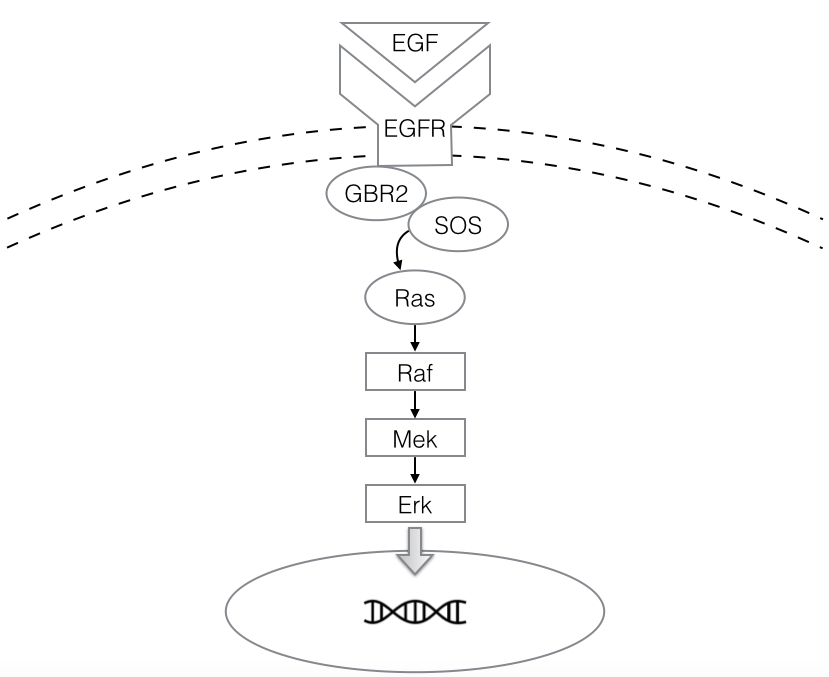
\includegraphics[width=0.4\textwidth]{figs/egfr.png}}
\caption{EGFR MAPK signaling pathway \cite{holbro2004erbb}, an example of a pathway containing the phosphorylation cascade from Raf to Mek to Erk.  The binding of ligand EGF to EGFR initiates a signal that leads to the cascade, which in turn regulates transcription.  This cascade implies two direct causal relationships, namely Raf --> MEK, and Mek --> Erk.  Raf and Erk have an indirect causal relationship, through Mek.\label{mapk}}
\end{figure}

Consider, e.g. the MAPK signaling cascade, which is part of several signaling pathways such as the EGFR MAPK pathway in Figure \ref{mapk}. In this cascade Raf causally affects the level of active (i.e., phosphorylated) Mek, while Mek causally affects Erk. Imagine these causal relationships were unknown: could they be detected from quantitative measurements on these phosphoproteins?  

To illustrate the process of causal inference in this context, we simulate artificial data using the computational Huang-Ferrell model of this cascade. The model represents the key binding, phosphorylation, and dephosphorylation reactions of the cascade with mass action kinetics, and replicates the MAPK key signaling behavior observed in nature.  With this model we simulated an experiment with 100 replicate biological samples, and measurements of concentration (umol) of phosphorylated Raf, and doubly phosphorylated Mek and Erk in each sample. 

\begin{figure}[!tpb]
\centerline{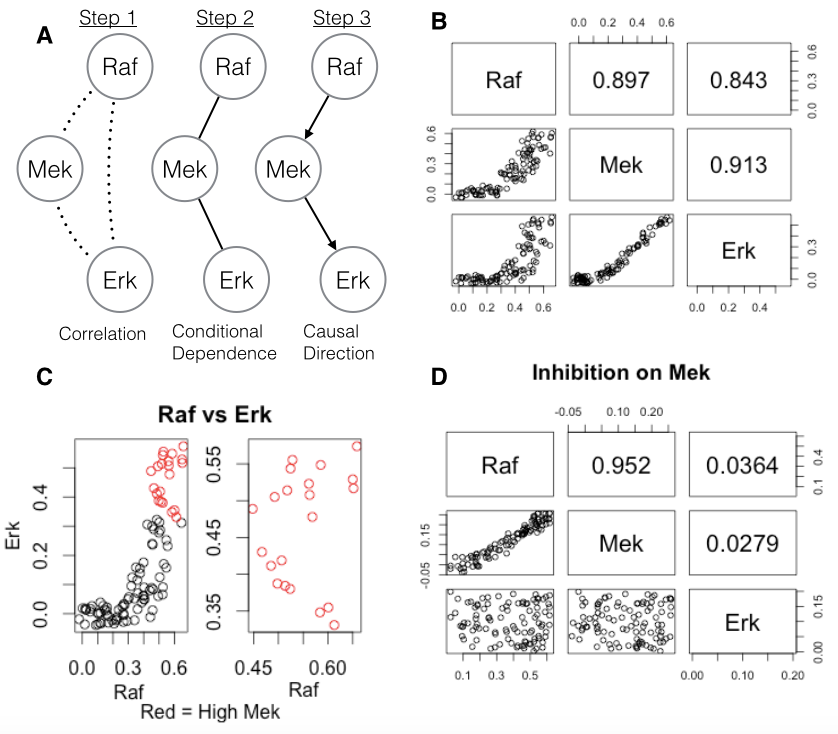
\includegraphics[width=1\textwidth]{figs/mapk.png}}
\caption{A: Overview of the 3 steps of causal inference, illustrated for the MAPK signaling cascade.    B, C, and D feature an experiment simulated from the Huang-Ferrell computational model of the phosphorylation cascade.  B: Pairwise plots of concentration values of phosphorylated (doubly phosphorylated for Mek and Erk) forms of each protein, and observed Spearman correlation values.  The Raf -- Erk correlation is high, despite the fact Raf does not directly regulate Erk.  C: Concentrations of Raf versus Erk, where samples corresponding to high Mek are highlighted in red.  In the right panel of B, only points with high levels of Mek are display (i.e. condition on Mek being high), and the observed association between Raf and Erk disappear, indicating Raf and Erk are conditionally independent given Mek.  D: After Raf is inhibited, the observed association between Raf and Mek remains while the association between Mek and Erk disappear.  Given Mek is conditionally dependent on Raf and on Erk, the inhibition reveals causal flow from Raf to Mek to Erk.}
\label{mapkInference}
\end{figure}


Figure \ref{mapkInference}A demonstrates the causal inference workflow starting with analysis of statistical associations in the data.  In step 1, a correlation graph between cascade components Raf, Mek, and Erk is assembled from the measurements of protein concentration.  Step 2 reduces the correlation graph to a sparse graph of conditional dependencies (Raf--Mek, and Mek--Erk).  Step 3 interrogates this graph to find putative causal relationships (Raf-->Mek, and Mek-->Erk).  While step 1 has little requirements, step 2 requires replicate biological samples, and step 3 requires systematic interventions (e.g. with protein inhibitors). 

Figure \ref{mapkInference}B illustrates Step 1 of the causal inference, and shows 2-way plots of the quantified protein concentrations, and Spearman correlations to quantify the extent of the associations.  The correlation values are high, and would meet most reasonable cut-off thresholds for constructing the correlation network in the left part of panel A.  The Raf--Mek and the Mek--Erk correlation edges match the Raf-->Mek, Mek-->Erk known causal edges.  What about the noncausal Raf--Erk edge? Despite the high Raf--Erk correlation, there is no direct causal mechanism between them (aside from the one via Mek, which is already accounted for via the Raf-->Mek and Mek-->Erk edges).  In causal  inference, our goal is to eliminate this "nuisance" edge.  How is this done?

To describe Step 2 of causal inference, we need some terminology. In statistical language, the quantified proteins are called {\it variables}. If the values of concentrations of two proteins vary between the biological samples in a coordinated manner, which is due to a common biological mechanism, the proteins are {\it statistically dependent}.  Just like the underlying biological mechanism is typically unknown, the presence of statistical dependence between two or more proteins is also unknown. Measures of statistical association (e.g.,  the Spearman correlation in Figure \ref{mapkInference}B or, alternatively, Pearson correlation or mutual information) demonstrate empirical evidence of the presence of such dependence. However, high associations are not a proof of direct causal relationships. In fact, the majority of statistical dependencies observed in experimental data reflect indirect associations. For example, a statistical association between an upstream and an indirect downstream protein can be due to the presence of intermediate proteins, such as the statistical association between Raf -- Erk is due to their indirect relationship through Mek. Another such example is a case where two proteins have a common regulator. In this case the two proteins are statistically associated through the regulator, without causally affecting one another. 

The direct causal events can be distinguished from other undesirable types of associations by controlling for (hold constant) the intermediaries and the common regulators. The absence of statistical association between two proteins, when the intermediates or the common regulators are controlled at a fixed level, is called {\it conditional independence}.  Causal inference searches for empirical evidence of conditional independence, to distinguish causal events from indirect associations. 

Let's see how this applies to the MAPK signaling cascade. We can examine the nature of statistical association between Raf and Erk.  Figure \ref{mapkInference}C compares Raf to Erk, highlighting in red the biological samples where concentrations of Mek are high (here, set to the top quartile).  Note that when we subset the data to only the red samples (in statistical language, when we condition on Mek being high), we can no longer detect the association between Raf and Erk. This has a mechanistic explanation. As can be seen in Figure \ref{mapk}, the abundance of Erk in each sample is determined by Mek. Therefore, when the abundance of Mek is fixed, Raf does not exert any additional influence on the variability of Erk.  This phenomenon -- the disappearence of the association between Raf and Erk upon conditioning on Mek - is evidence that  Raf and Erk are conditionally independent.  Once conditional independence is inferred from the data, the correlation edge arising from Raf--Erk dependence is removed, resulting in the middle graph of Figure \ref{mapk}A.

When the experiment quantifies all the key variables in a biological system, Step 2 above elucidates conditional dependence-based associations between causally related variables. In the MAPK example, this corresponds to a signaling protein's direct regulators, its direct effectors, and other proteins who share its direct effectors.  However, at this step the direction of the regulation remains unknown. Inference of the direction of the chain of events requires that the experimental design involves interventions. Figure \ref{mapkInference}D illustrates the results of Step 3, in the case of an intervention that targeted Mek with an inhibitor. With this intervention the concentration of Mek is unaffected, however its ability to phosphorylate other proteins is blocked.  After this intervention is introduced the Raf--Mek relationship is unchanged, while Erk drops to a low level.  From this we can infer that Mek has causal influence on Erk, and since Raf was unaffected by the intervention, that Raf has causal influence on Mek.  With the intervention, we can finally move from the conditional dependence graph in panel A - step 2 to the causal graph in panel A - step 3.

In the general case, computational methods for causal inference follow the workflow  in Figure \ref{mapkInference}A, while scaling it to characterize multiple inter-related variables. Step 1 creates a dense network of pairwise associations. Step 2 reduces this dense network to a sparse network of putative conditional dependencies, using empirical evidence of  conditional independence between pairs of variables. Finally, Step 3 uses the experimental design, specifically the information regarding the interventions, to evaluate these conditional dependencies as evidence for potential causal events.  See Koller-Friedman \cite{koller2009probabilistic} for a detailed description of these methods and their theoretical underpinnings. Several of these algorithms are implemented in the R package \textit{bnlearn} \cite{scutari2009learning}. 

\section{II. Large-scale statistical inference of causal relationships: challenges of scaling up}

A typical high-throughput experiments includes a small number of interventions, a small number of biological replicates, and a large number of analytes. This creates challenges in each of the 3 steps of causal inference above.

In Step 1, the challenge is in quantifying statistical associations between each pair of the analytes. A large number of proteins  leads to a large number of spurious statistical associations that arise without any biological justification, and purely as an artifact of random chance. Systematic pairwise relationships such as between Raf, Mek and Erk in the MAPK pathway will be obscured by the many spurious relationships that they will each form with causally unrelated proteins.

We illustrate this problem with a computer simulation, inspired by Fan et. al \cite{fan2014challenges} but translated to our context. First, we simulated an experiment that quantifies the abundances of 20 proteins in 100 biological samples.  Second, we simulates another experiment where the number of proteins was increased to 500.  In both experiments the proteins are completely independent from each other, and each protein in each replicate is assigned a value randomly drawn from a Gaussian distribution. In other words, we do not expect any biologically meaningful associations in these data. We repeated each of these simulations 500 times. Figure \ref{spur_corr} plots the histograms of the highest Pearson correlation found across any pair of proteins in the 500 simulations, separately for each experiment. As can be seen, the experiment with 500 proteins produces relatively large maximum pairwise correlations, demonstrating that an increase in the number of proteins leads to an increase in spurious correlations.  This is a clearly problem when high correlation is used as an initial evidence of a biological function.


\begin{figure}[!tpb]
\centerline{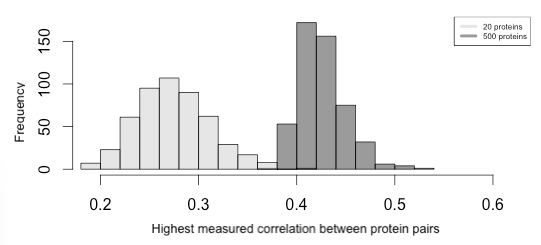
\includegraphics[width=1\textwidth]{figs/spurious_corr.png}}
\caption{Simulated experiments quantifying 20 (or 500) unrelated proteins in 100 biological samples, each repeated 500 times. The plots are the histograms of the highest Pearson correlation found across any pair of proteins, calculated over the 500 simulations. Increasing the number of proteins results in higher spurious associations.}
\label{spur_corr}
\end{figure}

Similarly, the increased incidence of spurious correlations impedes the performance of statistical methods in Step 2, which elucidate conditional independences in the data.  The spurious correlations result in more false positives when detecting putative causal conditional dependence relationships. To illustrate, we repeated the previous simulation, again starting with 20 proteins and 100 biological samples, but this time expanding to only 100 proteins.  Instead of finding the highest  spurious correlation between pairs of proteins, we apply the a causal inference-related algorithm described in Margaritis 2003 \cite{margaritis2003learning}, which performs a series of conditional independence tests between the sets of proteins, and count the number of detected conditional dependence relationships.  As before, since we randomly draw protein abundance measurement values from a Gaussian distribution, the values are completely independent, and any conditional dependence relationship reported by this algorithm has no biological justification.  We again repeat these experiments 500 times. Figure \ref{spur_dep} shows the histograms of the counts of false positive detections of conditional dependence.  The results demonstrate that an increase in the number of proteins leads to an increase in false positive detection of putative causal conditional dependence relationships. This means that the computational methods for causal inference will fail for a typical large-scale experiment, because they cannot reliably detect the conditional dependence relationships needed to infer causality.

\begin{figure}[!tpb]
\centerline{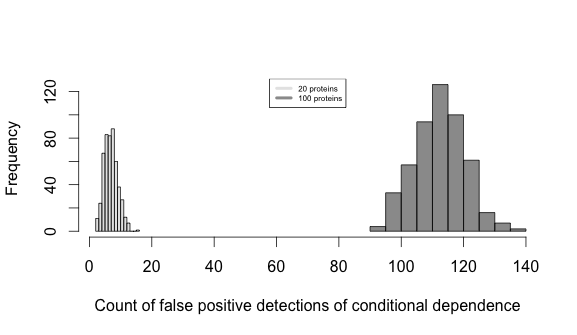
\includegraphics[width=1\textwidth]{figs/spurious_dep.png}}
\caption{As in Figure \ref{spur_corr}, but reporting the counts of false positive detections of conditional dependence.}
\label{spur_dep}
\end{figure}

An additional problem for Step 2 is a typically small number of biological replicates that these experiments have as compared to the number of analytes. While Step 1 (evaluating the set of pairwise associations) can be carried out with even a small amount of replicates, Step 2 requires that the number of replicates is equal or exceeds the number of analytes.  Note the experiments demonstrated in Figure 3 had 100 replicates to its 100 proteins. This number of samples per analyte is much larger than in a typical high-throughput experiment.  While sparse approaches working around ths problem are available, quality of their results decreases drastically as the number of replicates fall.    

Finally, Step 3 of the workflow requires interventions to infer causal relationships from evidence of conditional dependence.  Quantifying a large number of analytes introduces a  challenge for this step as well. As the number of features grows, the number of interventions needed to fully infer causality grows, and eventually performing a sufficient perturbation experiments becomes infeasible.   We showed with Raf-Mek-Erk example that one intervention was sufficient to infer two causal relationships, and indeed when measuring $k$ variables a set of interventions on $< k$ variables may be sufficient to infer causality.  But along with having too few replicates, the typical large-scale experiment has far too few interventions.  Also, if the step 2 results in too many false positives for conditional dependence, this will adversely affect the results of step 3 regardless of the size of the set of interventions.


\section{III. Approaches for inferring causality from high-throughput experiments}

The problems outlined in section II paint a grim picture for causal learning in large datasets. Fortunately, these can be overcome, and effective causal learning can be a reality for large scale datasets.  We describe best practices  in the Causality Inference in Omics  below.


\begin{enumerate}
\item \textit{Limiting the number of analytes}, and use a small subset of biologically relevant and technologically accurate measurements. The length of the list of identified and quantified analytes is not as important as the focus of the investigation and the quality of measurements on important parts of the system.  If the broader biological system is well understood, it may be possible design to a targeted experiment that focuses on a specific part of the system of interest, then ask more distinct questions of the data, such as whether a particular edge or pathway is present.  The more specific the question, the less data needed overall to make solid causal inference.  
\item \textit{Measure more samples}.  If feasible, high throughput measurements that measure many samples (not just many proteins) provide the statistical power to distinguish true associations from spurious associations.  This intuition motivates the use of technologies that measure fewer variables but enable measurement of more samples (or gather more data points per sample), for causal modeling.  A related  example is  use of single cell data for inference (e.g. from single cell  mass cytometry), where  many thousands of cells per sample provide ample statistical power. See Sachs et al 2005 for an in depth case study. \cite{sachs2005causal}
\item \textit{Use prior knowledge}, not just from experts but also from noisier sources, to improve the process of searching for conditional independence.  The MAPK pathway for instance, mentioned earlier, is canonical and well established.  The process of inferring causal connections is helped by assuming a priori that such canonical connections exist. This is because knowledge of parts of the underlying regulatory network reduces the remaining number of possible associations, and enables more effective use of data. The number of total associations examined goes down, enabling increased confidence in statistical associations that are found.  Knowledge about canonical causal relationships can be sourced from pathway databases such as KEGG. Another example of prior knowledge is contextual information, such as spatial relations between  signaling proteins in the cell -- causal inference algorithms can be formulated to weigh evidence of conditional dependence differently depending on whether proteins are from the same or different spatial compartments. 
\item \textit{Employ targeted interventions selectively}. Targeted interventions perturb individual components of the system.  An example is small molecule inhibitors which block the causal influence of a specific protein on downstream components.  Since it is usually prohibitive to perturb every target component of a system, it is strategic to prioritize application of targeted interventions to parts of the system that have the most potential for new discoveries.  Selection of these perturbation targets can be based on prior knowledge - e.g. knowledge of which components are crucial players in the system of interest - or they can be applied iteratively, after an initial statistical analysis has revealed areas of the network in which causal inferences are not possible based on existing data.  For instance, a resulting model graph with undirected edges can be inspected to reveal which nodes have potential to reveal the most causality if perturbed.
\item \textit{Consider broad-scale interventions}. Traditionally, experiments characterize a biological response to a particular stimulus, possibly in the context of an inhibitor.  In contrast, broad-scale interventions sacrifice specificity to perturb many features in the system simultaneously.  The advantage of this approach is that it may enable elucidation of  causality across the entire system.  Just as one intervention was sufficient to infer causality between three proteins (Raf, Mek, and Erk), perturbing many things at once creates cascades of causal direction orientation across the broader network.  This includes varying experimental conditions to activate multiple pathways.  For example, signals from endocrine, paracrine, and autocrine ligands elicit various signaling responses in hepatocytes, thus interventions that cover this range of signals gives the best picture of the broader causal network of hepatocyte signaling.  Similarly, interventions that go beyond receptor-level and perturb multiple components of the system bring cascading causal direct orientation deeper into the network.  Although they do not provide specific information about the downstream effects of stimulation,  broad-scale interventions can provide more causal inference bang for your intervention buck.   

\end{enumerate}

\textit{The Causality in Omics Tool List} above provides impactful approaches
that can drastically improve causal inference from omics datasets, by
constraining the inference task, and thus allowing for accurate
statistical inferences. For instance, the task of assessing which of all
the possible KEGG pathways is present in a dataset will be far less
error-prone than the task of assessing which of all possible
combinations of my measured features might form a biological pathway.

How should the tools listed be used? They are most powerful when used in
combination, and in fact the lines between them are somewhat arbitrary
and frequently blurred. For instance, using tool \#1 and tool \#2 in
concert can be thought of as reducing the breadth and increasing the
depth of the investigation. Tools \#4 and \#5 call for use of
interventions, but this task itself is complicated by measuring many
things, since we have more features to expose to intervention. Tool
\#3, prior biological knowledge, can be used to prioritize what to
target with that limited set of interventions.  Causal inference becomes possible when using these tools in combination with a sound experimental design.

\begin{acknowledgement}
We acknowledge the participants of Dagstuhl seminar 15351 "Computational Mass Spectrometry" (December 2015) (http://www.dagstuhl.de/de/programm/kalender/semhp/?semnr=15351) for their contributions to the discussion on computational manuscripts.
\end{acknowledgement}
\bibliography{write_up}
\end{document}
